\documentclass[a4paper, 12pt]{article}

\usepackage[no-math]{fontspec-xetex}
\setmainfont{IBM Plex Sans}
\usepackage[english, russian]{babel}

\usepackage{blindtext}
\usepackage{microtype}
\usepackage{geometry}

\usepackage{amsmath, amsfonts, amssymb, amsthm, mathtools}
\usepackage{MnSymbol}
\usepackage{physics}

\usepackage{graphicx, wrapfig, caption, subcaption}
\usepackage{color, xcolor}

\usepackage{titlesec}
\usepackage[document]{ragged2e}
\usepackage{enumitem}
\usepackage{hyperref}
\usepackage{import}

\graphicspath{{figures/}}
\geometry{margin=6em}
\geometry{bottom=6em}

% Настройки заголовков
\titleformat{\section}[hang]{\Large}{}{0em}{}{}
\titleformat{\subsection}[hang]{\large}{}{0em}{}{}

% Настройки параграфов текста
\setlength{\parindent}{0em}
\setlength{\parskip}{1em}
\renewcommand{\baselinestretch}{1.1}

% Настройки списков
\setlist{leftmargin=*, noitemsep}

% Настройки таблиц
\setlength{\tabcolsep}{2em}
\renewcommand{\arraystretch}{1.3}

% Настройки ссылок
\hypersetup{colorlinks=true, linkcolor=blue, urlcolor=blue}

\title{Модуль сдвига и крутильные колебания}
\author{Роман Ухоботов, Николай Грузинов}
\date{}%собрано \today}

\begin{document}
\maketitle

\section{Используемое оборудование}
\begin{enumerate}
\item динамометр (max $1$~Н, цена деления $0.02$~Н);
\item 8 стержней разных длин, масс, диаметров и материалов;
\item крутящаяся платформа с встроенным транспортиром;
\item 2 груза для изменения момента инерции платформы;
\item оптические ворота (для измерения периода, погрешность: $0.01$~c);
\end{enumerate}

\section{Цели и задачи}
Цель: изучить крутильные колебания различных стержней, измеряя период колебаний и крутильный коэффициент жесткости.
Задачи:
\begin{enumerate}
\item измерить момент инерции крутящейся платформы без грузов
\item измерить диаметры стержней (точнее, чем в паспорте) и массы грузов
\item для каждого из восьми стержней измерить динамометром крутильный коэффициент жесткости в статике.
\item для каждого стержня измерить период колебаний оптическими воротами
\item среди стержней есть 3 стержня из одного материала и одного диаметра, но разной длины --- посмотреть на зависимость периода колебаний и крутильного коэффициента жесткости от длины;
\item есть два стержня из одного материала и одинаковой длины, но разных диаметров --- посмотреть на зависимость от диаметра;
\item вычислить модуль сдвига (или модуль Юнга) стали, алюминия, меди и латуни; сравнить c табличными значениями. 
\end{enumerate}

\section{Теоретическая модель}
В первом приближении для крутильных колебаний работает ``закон Гука'': момент силы $M$ пропорционален углу поворота платформы $\alpha$ c крутильным коэффициентом жесткости $k$.
Колебания платформы на стержне описываются вторым законом Ньютона для вращательного движения, что позволяет легко связать период колебаний $T$, момент инерции платформы (с грузами или без) $I$ и крутильный коэффициент жесткости $k$:
\[ M = I \beta \quad\implies\quad -k\alpha = I \ddot{\alpha} .\]
Крутильный коэффициент жесткости $k$ связан с модулем сдвига $G$ уравнением
%TODO: посчитать интеграл из методички тут
\[ k = \frac{\pi d^4 G}{32l} \tag{$d$ --- диаметр, $l$ --- длина стержня} .\]
Также известна связь модуля сдвига $G$ с модулем Юнга $E$ и коэффициеентом Пуассона $\nu$:
\[ G = \frac{E}{2(1 + \nu)} .\]
Моменты инерции при добавлении грузов складываются: если момент инерции платформы без дополнительных грузов $I_0$, масса одного груза $m$, продольная длина груза $b$, а расстояние от оси до центра груза $a$, то суммарный момент инерции составит
\[
I = I_0 + 2 \frac{m}{b} \int\limits_{a - \frac{b}{2}}^{a + \frac{b}{2}} r^2 \dd r =
    I_0 + \frac{2m}{3b} \bigl( (a + \tfrac{b}{2})^3 - (a - \tfrac{b}{2})^3 \bigr) =
    %I_0 + \frac{2m}{3b} \bigl( a^3 + \tfrac{1}{8} b^3 + \tfrac{3}{2} a^2 b + \tfrac{3}{4} ab^2 -
    %                          (a^3 - \tfrac{1}{8} b^3 - \tfrac{3}{2} a^2 b + \tfrac{3}{4} ab^2)\bigr)
    %I_0 + \frac{2m}{3b} \bigl( \tfrac{1}{4} b^3 + 3a^2 b \bigr)
    I_0 + 2m \left( a^2 + \frac{b^2}{12} \right)
    %I_0 + 2m a^2 + \frac{mb^2}{6}
.\]

\section{Методика измерений}
Диаметр $d$ стержней измеряли микрометром, параметры $a$ и $b$ для грузов --- линейкой.
Коэффициент $k$ в статике получали косвенно измерением 5--6 точек зависимости силы от угла, тянув динамометром за плечо платформы.
Период колебаний измерялся в соответствующем режиме оптическими воротами.

\section{Результаты}
Массы грузов $m_1 = 152.75$~г, $m_2 = 151.95$~г, $\Delta m = 0.01$~г.
Будем считать, что в формуле для момента инерции $2m = m_1 + m_2 = 304.70 \pm 0.02$~г.
Продольная длина груза $b = 3.0 \pm 0.1$~см.
Расстояние от оси до центра груза $a = 15 \pm 0.3$~см.

\begin{table}[!htbp]
\label{tab:force-angle}
\caption{
    Измерения динамометром для стержней 1-8, слева направо, снизу вверх.
    Плечо, за которое тянули --- $a$.
}
\begin{tabular}{ll}
\hline
 Сила, Н & Угол, $^\circ$ \\
 0.0     & 1.0            \\
 0.3     & 10.0           \\
 0.5     & 17.0           \\
 0.6     & 19.0           \\
 0.9     & 30.0           \\
 1.0     & 34.0           \\
\hline
\end{tabular}
\begin{tabular}{|c|c|}
\hline
Сила, Н & Угол, $^\circ$ \\ \hline
0.00 & 0 \\ \hline
0.30 & 29 \\ \hline
0.50 & 48 \\ \hline
0.80 & 80 \\ \hline
1.00 & 100 \\ \hline
\end{tabular}

\begin{tabular}{ll}
\hline
 Сила, Н & Угол, $^\circ$ \\
 0.0     & 0.0            \\
 0.3     & 23.0           \\
 0.5     & 40.0           \\
 0.7     & 58.0           \\
 0.9     & 79.0           \\
\hline
\end{tabular}
\begin{tabular}{|c|c|}
\hline
Сила, Н & Угол, $^\circ$ \\ \hline
0.00 & 0 \\ \hline
0.30 & 18 \\ \hline
0.60 & 36 \\ \hline
0.90 & 55 \\ \hline
1.00 & 61 \\ \hline
\end{tabular}

\begin{tabular}{|c|c|}
\hline
Сила, Н & Угол, $^\circ$ \\ \hline
0.00 & 0 \\ \hline
0.30 & 6 \\ \hline
0.60 & 12 \\ \hline
0.90 & 19 \\ \hline
1.00 & 21 \\ \hline
\end{tabular}

\begin{tabular}{|c|c|}
\hline
Сила, Н & Угол, $^\circ$ \\ \hline
0.00 & 0 \\ \hline
1.00 & 6 \\ \hline
1.40 & 9 \\ \hline
1.60 & 10 \\ \hline
2.00 & 13 \\ \hline
\end{tabular}

\begin{tabular}{|c|c|}
\hline
Сила, Н & Угол, $^\circ$ \\ \hline
0.00 & 0 \\ \hline
0.20 & 14 \\ \hline
0.40 & 30 \\ \hline
0.60 & 44 \\ \hline
0.80 & 63 \\ \hline
\end{tabular}

\begin{tabular}{|c|c|}
\hline
Сила, Н & Угол, $^\circ$ \\ \hline
0.00 & 0 \\ \hline
0.20 & 10 \\ \hline
0.40 & 21 \\ \hline
0.60 & 34 \\ \hline
0.80 & 48 \\ \hline
\end{tabular}

\end{table}

\begin{figure}
\label{fig:torque-angle-plot}
\begin{center}
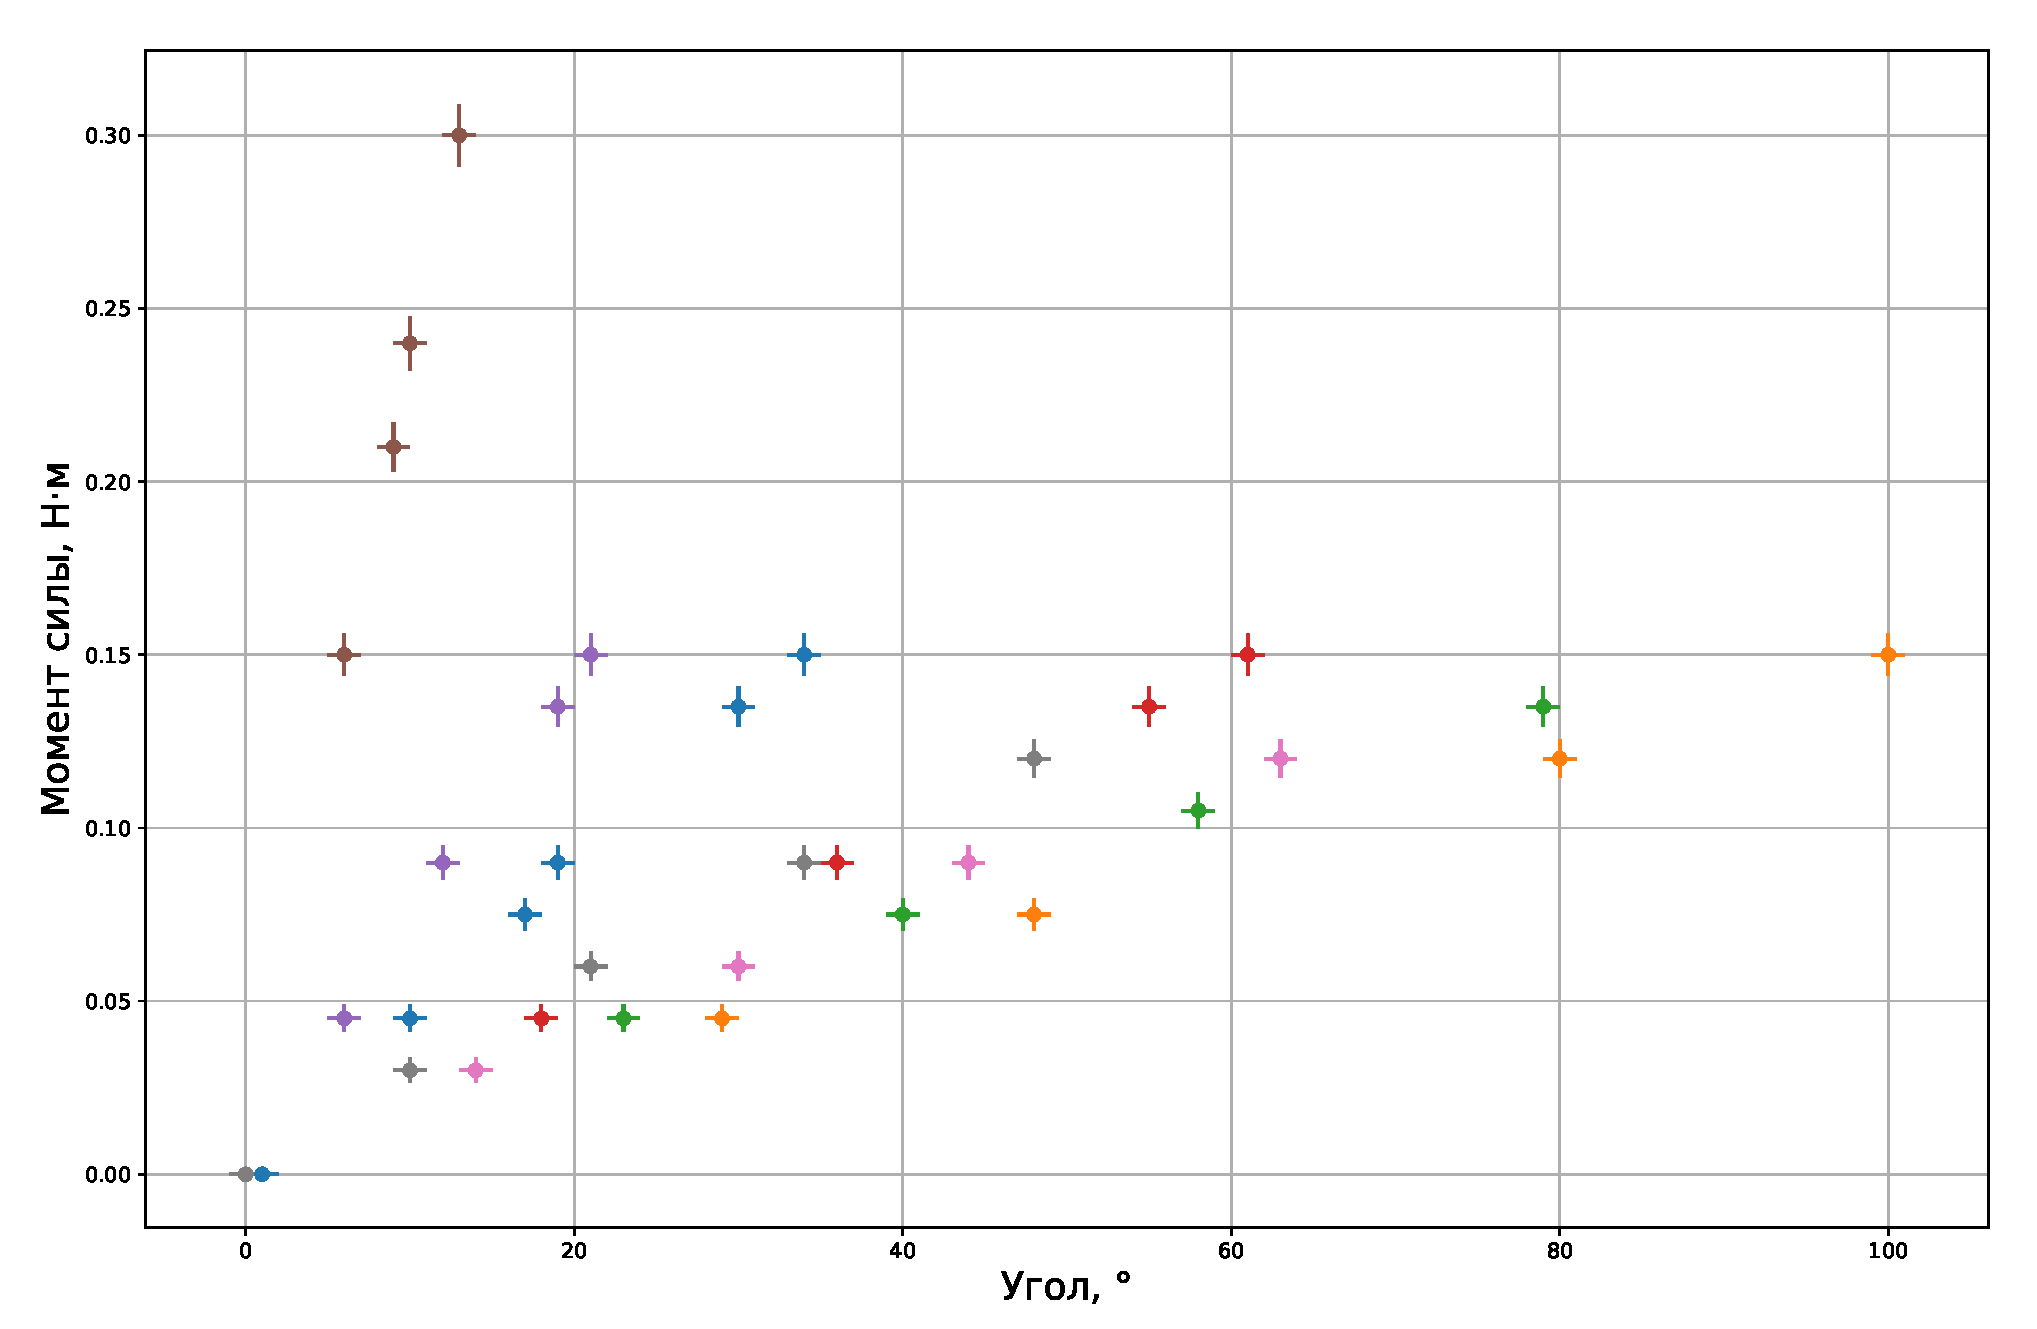
\includegraphics[width=0.9\linewidth]{torque-angle-plot.pdf}
\end{center}
\end{figure}

%\section{Выводы}
\end{document}
